\documentclass[11pt]{article}
%\usepackage[firstpage]{draftwatermark}
\usepackage{times}
\usepackage{pdfpages}
\usepackage{fullpage}
\usepackage{url}
\usepackage{hyperref}
\usepackage{fancyhdr}
\usepackage{graphicx}
\usepackage{tabularx}
\usepackage{enumitem}
\usepackage{indentfirst}
\usepackage{subcaption}
\usepackage{amsmath, amssymb}
\DeclareMathOperator*{\argmax}{arg\,max}
\DeclareMathOperator*{\argmin}{arg\,min}
\usepackage{units}
\usepackage{IEEEtrantools}

% Added by bsb
\usepackage{color,soul}
\DeclareRobustCommand{\hlr}[1]{{\sethlcolor{red}\hl{#1}}}
\DeclareRobustCommand{\hlg}[1]{{\sethlcolor{green}\hl{#1}}}
\DeclareRobustCommand{\hlb}[1]{{\sethlcolor{blue}\hl{#1}}}
\DeclareRobustCommand{\hly}[1]{{\sethlcolor{yellow}\hl{#1}}}

\setcounter{secnumdepth}{4}
\graphicspath{{images/}}
\pagestyle{fancy}

\newcommand{\doctitle}{Modeling single-beam sonar with Gazebo ray tracing}

\addtolength{\headheight}{2em}
\addtolength{\headsep}{1.5em}
\lhead{\doctitle}
\rhead{}

\newcommand{\capt}[1]{\caption{\small \em #1}}

\cfoot{\small Brian Bingham \today \\ \thepage}
\renewcommand{\footrulewidth}{0.4pt}

\newenvironment{xitemize}{\begin{itemize}\addtolength{\itemsep}{-0.75em}}{\end{itemize}}
\newenvironment{tasklist}{\begin{enumerate}[label=\textbf{\thesubsubsection-\arabic*},ref=\thesubsubsection-\arabic*,leftmargin=*]}{\end{enumerate}}
\newcommand\todo[1]{{\bf TODO: #1}}
\setcounter{tocdepth}{2}
\setcounter{secnumdepth}{4}

\makeatletter
\newcommand*{\compress}{\@minipagetrue}
\makeatother

%\renewcommand{\chaptername}{Volume}
%\renewcommand{\thesection}{\Roman{section}}
%\renewcommand{\thesubsection}{\Roman{section}-\Alph{subsection}}

\begin{document}

% More verticle spacing in eqnarray
\setlength{\IEEEnormaljot}{10pt}%


% set the figure default size
\newcommand{\SF}{0.7}
\newcommand{\SFb}{0.45}
\newcommand{\SFPic}{0.45}
\newcommand{\SFPlot}{0.45}
\newcommand{\SFc}{0.52}
% Just a lazy way of setting the figure width (percentage of text width)
% 0.7 works well for 1 column
% 0.4 works well for 2 column
\newcommand{\FigWidth}{\SF}


\newpage
% Title Page
\setcounter{page}{1}
\begin{center}
{\huge \doctitle}\footnote{Document source at \url{https://www.overleaf.com/read/tcxjgnmqphwj} and \url{https://github.com/bsb808/OceanNotes}}
\end{center}

%\begin{abstract}
%Abstract
%\end{abstract}

\section{Sonar Model}

The echo level is
\begin{equation}
EL = SL - 2(TL)+ TS % = 10 \log\left( \frac{I_R}{I_T} \right)
\end{equation}
where SL is the source level, TL is the transmission loss, TS is target strength, $I_R$ is the reflected intensity and $I_T$ is the transmitted intensity.  To start with we use the \verb+laser_retro+ method to provide the reflected intensity.

\section{Beam Pattern Model}

The background of modeling the beam pattern is covered by the following:
\begin{itemize}
\item \href{http://www.personal.psu.edu/faculty/m/x/mxm14/}{Martin Mazur's} 2012 Underwater Acoustics (Penn State) \href{http://www.personal.psu.edu/faculty/m/x/mxm14/sonar/Mazur-sonar_signal_processing_combined.pdf}{course notes}.
\item John Leonard's \href{https://ocw.mit.edu/courses/mechanical-engineering/2-011-introduction-to-ocean-science-and-engineering-spring-2006/readings/hw5_sonar_leonar.pdf}{Introduction to Sonar} from Alex Techet's 2006 Introduction to Ocean Science and Engineering \href{https://ocw.mit.edu/courses/mechanical-engineering/2-011-introduction-to-ocean-science-and-engineering-spring-2006/}{course notes}.
\item \href{https://www3.mbari.org/data/mbsystem/sonarfunction/SeaBeamMultibeamTheoryOperation.pdf}{SeaBeam Multibeam Sonar Theory of Operation}.
\end{itemize}

\subsection{Beam Pattern Geometry}
The geometry of the beam pattern is illustrated in Figure~\ref{f:bpattern}.  Most of the energy in the beam pattern is in the \emph{main lobe} and the center of that lobe is the \emph{main response axis} (MRA), shown as the Main axis in the figure. The angle from the MRA to the \emph{half power point} is $\theta_w$ and the \emph{beam width} (Full angle in the Figure) is twice this value:
\begin{equation}
\theta_{bw}=2 \theta_w
\end{equation}

\begin{figure}[hbt!]
  \centering
  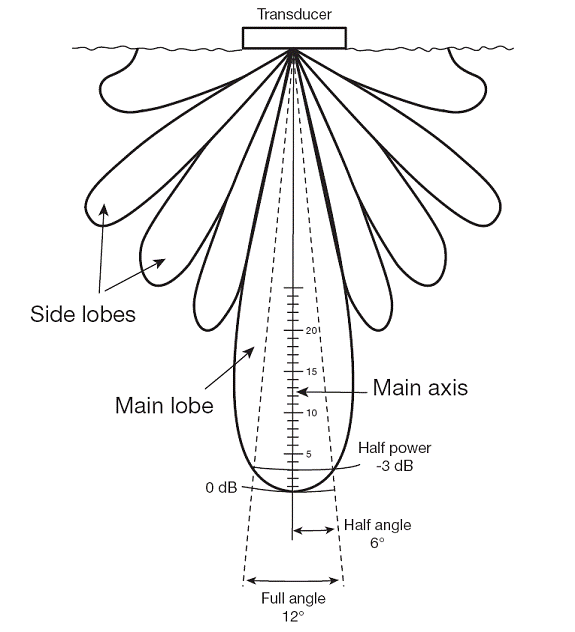
\includegraphics[width=0.4\textwidth]{images/beampattern.png}
  \caption{Beam pattern schematic from \url{http://www.acousticsunpacked.org/AcousticBackground/AcousticTransducers.html}}
  \label{f:bpattern}
\end{figure}
The beam pattern expresses the echo level as a function $\theta$, the angle relative the the MRA, as
\begin{equation}
EL = \left| G(\theta) \right|^2
\end{equation}

\subsection{Line Array Beam Pattern}
For a line array of length $L$, radiating energy at wavelenth $\lambda$, the beam pattern is that of the \emph{uniform aperature function}.  The radiated power is modeled as a \emph{normalized sinc function}
\begin{equation}
\left| G(L u) \right|^2 =  \left|\mathrm{sinc}(L u)\right|^2 = 
\begin{cases}
  1 & \text{for} \, \,  Lu = 0 \\
 \left| \frac{\sin(\pi L u)}{\pi L u} \right|^2  & \text{otherwise}
  \end{cases}
\end{equation}
where $u$ is the \emph{electrical angle}
\begin{equation}
u = \frac{\sin(\theta)}{\lambda}.
\end{equation}
We can solve for the half power point by setting
\begin{equation}
G(\theta_w) = \frac{\sin(\pi \frac{L}{\lambda} \sin(\theta_w))}{\pi \frac{L}{\lambda} \sin(\theta_w)} = \frac{1}{\sqrt{2}}.
\end{equation}
For conditions where $L >> \lambda$, which is typical of high-frequency sonar, the half power point is
\begin{equation}
\theta_{w} = 0.442 \frac{\lambda}{L} \,\, \unit[]{rad}.
\end{equation}
When given a beam width, $\theta_{bw} = 2 \theta_w$ we can solve for the length to wavelength ratio
\begin{equation}
\frac{L}{\lambda} = \frac{0.884}{\theta_{bw}} = \frac{0.442}{\theta_w}
\end{equation}
so that the beam pattern is
\begin{equation}
\left| G(\theta_w) \right|^2 = \left| \frac{\sin(\pi \frac{0.884}{\theta_{bw}} \sin(\theta))}{\pi \frac{0.884}{\theta_{bw}} \sin(\theta)} \right|^2
\end{equation}
where $\theta_{bw}$ is the beam width in radians.  Figures \ref{f:linebp_polar} and \ref{f:linebp}\footnote{Figure Python source code at \url{https://bitbucket.org/brian_bingham/ocean_notes/src/master/src/single_beam/beam_pattern.py}} illustrate this beam pattern for a range of $L/\lambda$ values.  The differences in the beam shape between $[-\theta_w,\theta_w]$ is sufficiently small to be neglected.

\begin{figure}[hb!]
  \centering
  \begin{subfigure}[t]{0.5\textwidth}
    \centering
    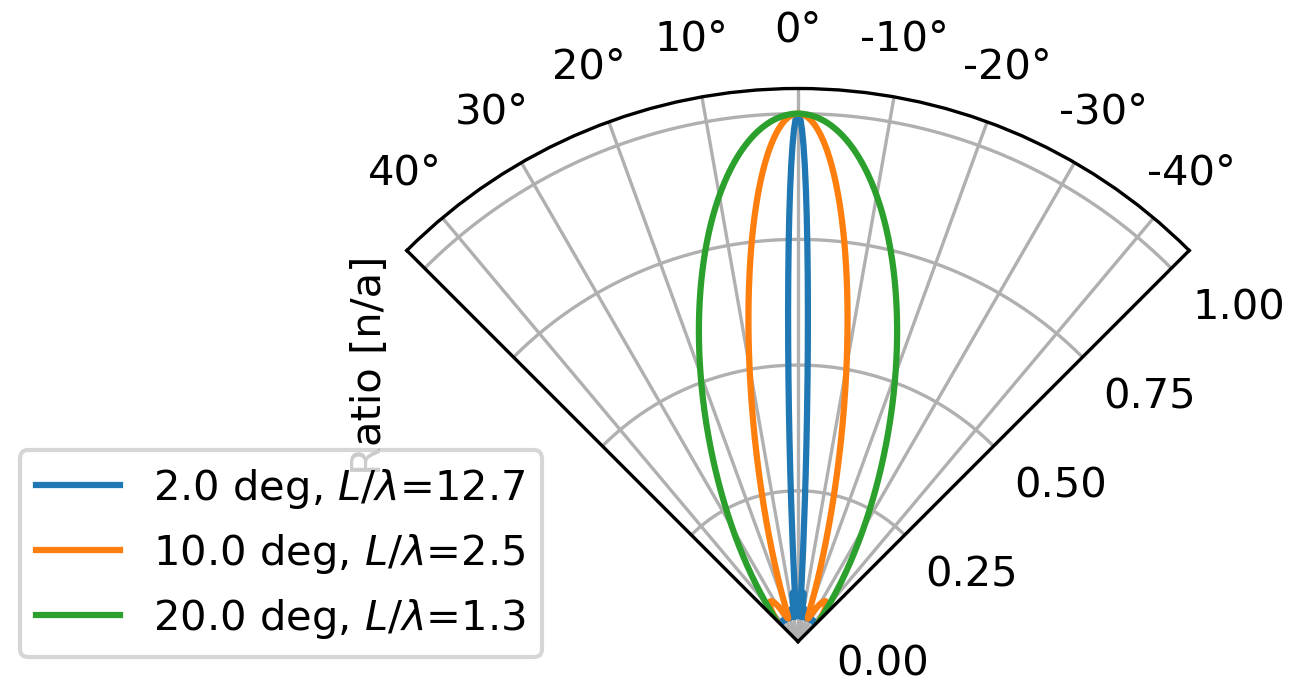
\includegraphics[width=\textwidth]{src/single_beam/linebp_polar_ratio_c.png}
    \caption{As ratio.}
  \end{subfigure}%
  ~ 
  \begin{subfigure}[t]{0.5\textwidth}
    \centering
    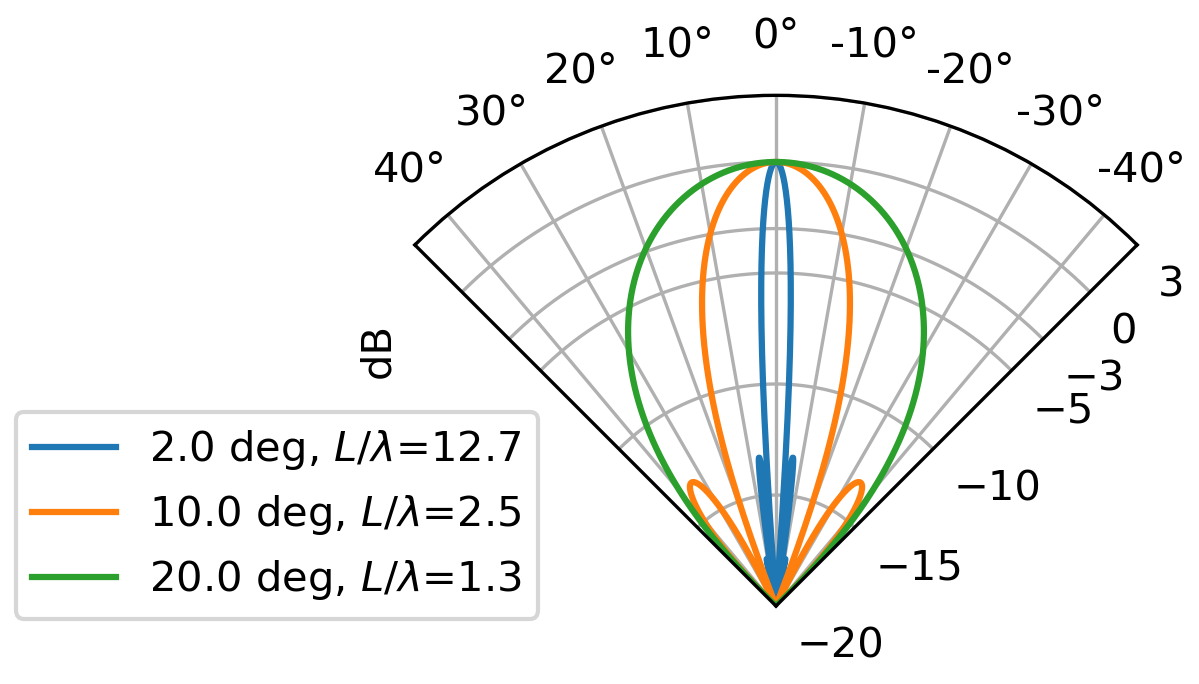
\includegraphics[width=\textwidth]{src/single_beam/linebp_polar_db_c.png}
    \caption{In dB.}
  \end{subfigure}
  \caption{Beam pattern in polar coordinates. }
  \label{f:linebp_polar}
\end{figure}


\begin{figure}[hb!]
  \centering
  \begin{subfigure}[t]{0.5\textwidth}
    \centering
    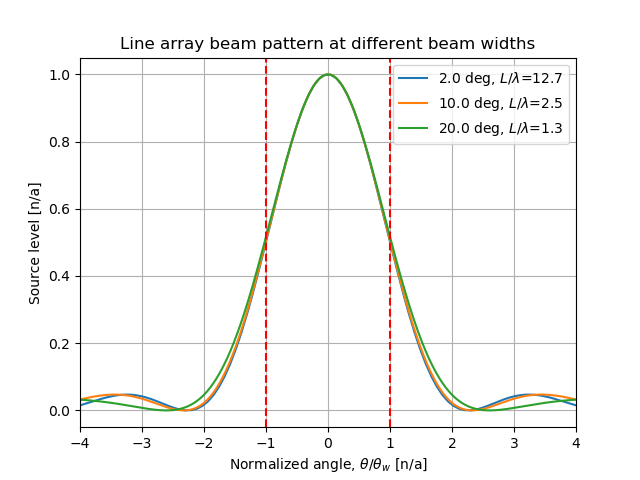
\includegraphics[width=\textwidth]{src/single_beam/linebp_ratio.png}
    \caption{As ratio.}
  \end{subfigure}%
  ~ 
  \begin{subfigure}[t]{0.5\textwidth}
    \centering
    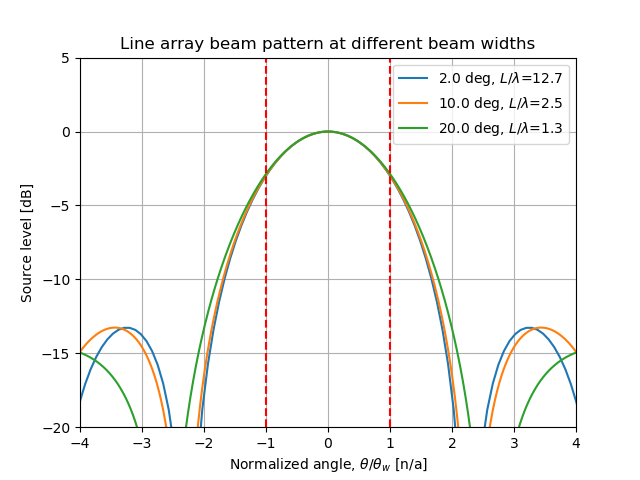
\includegraphics[width=\textwidth]{src/single_beam/linebp_db.png}
    \caption{In dB.}
  \end{subfigure}
  \caption{Beam pattern in Cartesian coordinates. }
  \label{f:linebp}
\end{figure}

\subsection{Sampling the Beam Pattern via Ray Tracking}

For a single beam sonar the model generates a single range and intensity pair: $(\bar{r},\bar{i})$.  We generate this pair by a uniform sampling of the beam pattern as shown in Figure~\ref{f:bpsampled}.  Each sample is a ray at $\theta_k$ in the range $[-\theta_w, \theta_w]$ generating the range/intensity pair $(r_k,i_k)$.  The set of ordered pairs from all the rays is $R = \{(r_0,i_0),(r_1,r_1),\ldots,(r_N,i_n)\}$.

\subsubsection{Beam Echo Level - Intensity}

The intensity value for each ray is the echo level for that geometry, $i_k = EL_k$.  We use a weighted average to model the beam pattern effect
\begin{equation}
\bar{EL} = \bar{i} = \frac{ \sum_{k=0}^{N} w_k i_k }{\sum_{k=0}^N w_k}
\end{equation}
where the weights are determined from the beam pattern function
\begin{equation}
w_k = \left| G(\theta_k) \right|^2 = \left| \frac{\sin(\pi \frac{0.884}{\theta_{bw}} \sin(\theta_k))}{\pi \frac{0.884}{\theta_{bw}} \sin(\theta_k)} \right|^2
\end{equation}

\subsubsection{Beam Range}
The single-beam range value is the ray length corresponding to the maximum intensity, i.e.,\footnote{Need to improve notation here.}
\begin{equation}
(\bar{r},i_{max}) = \max(R)
\end{equation}


\begin{figure}[hbt!]
  \centering
  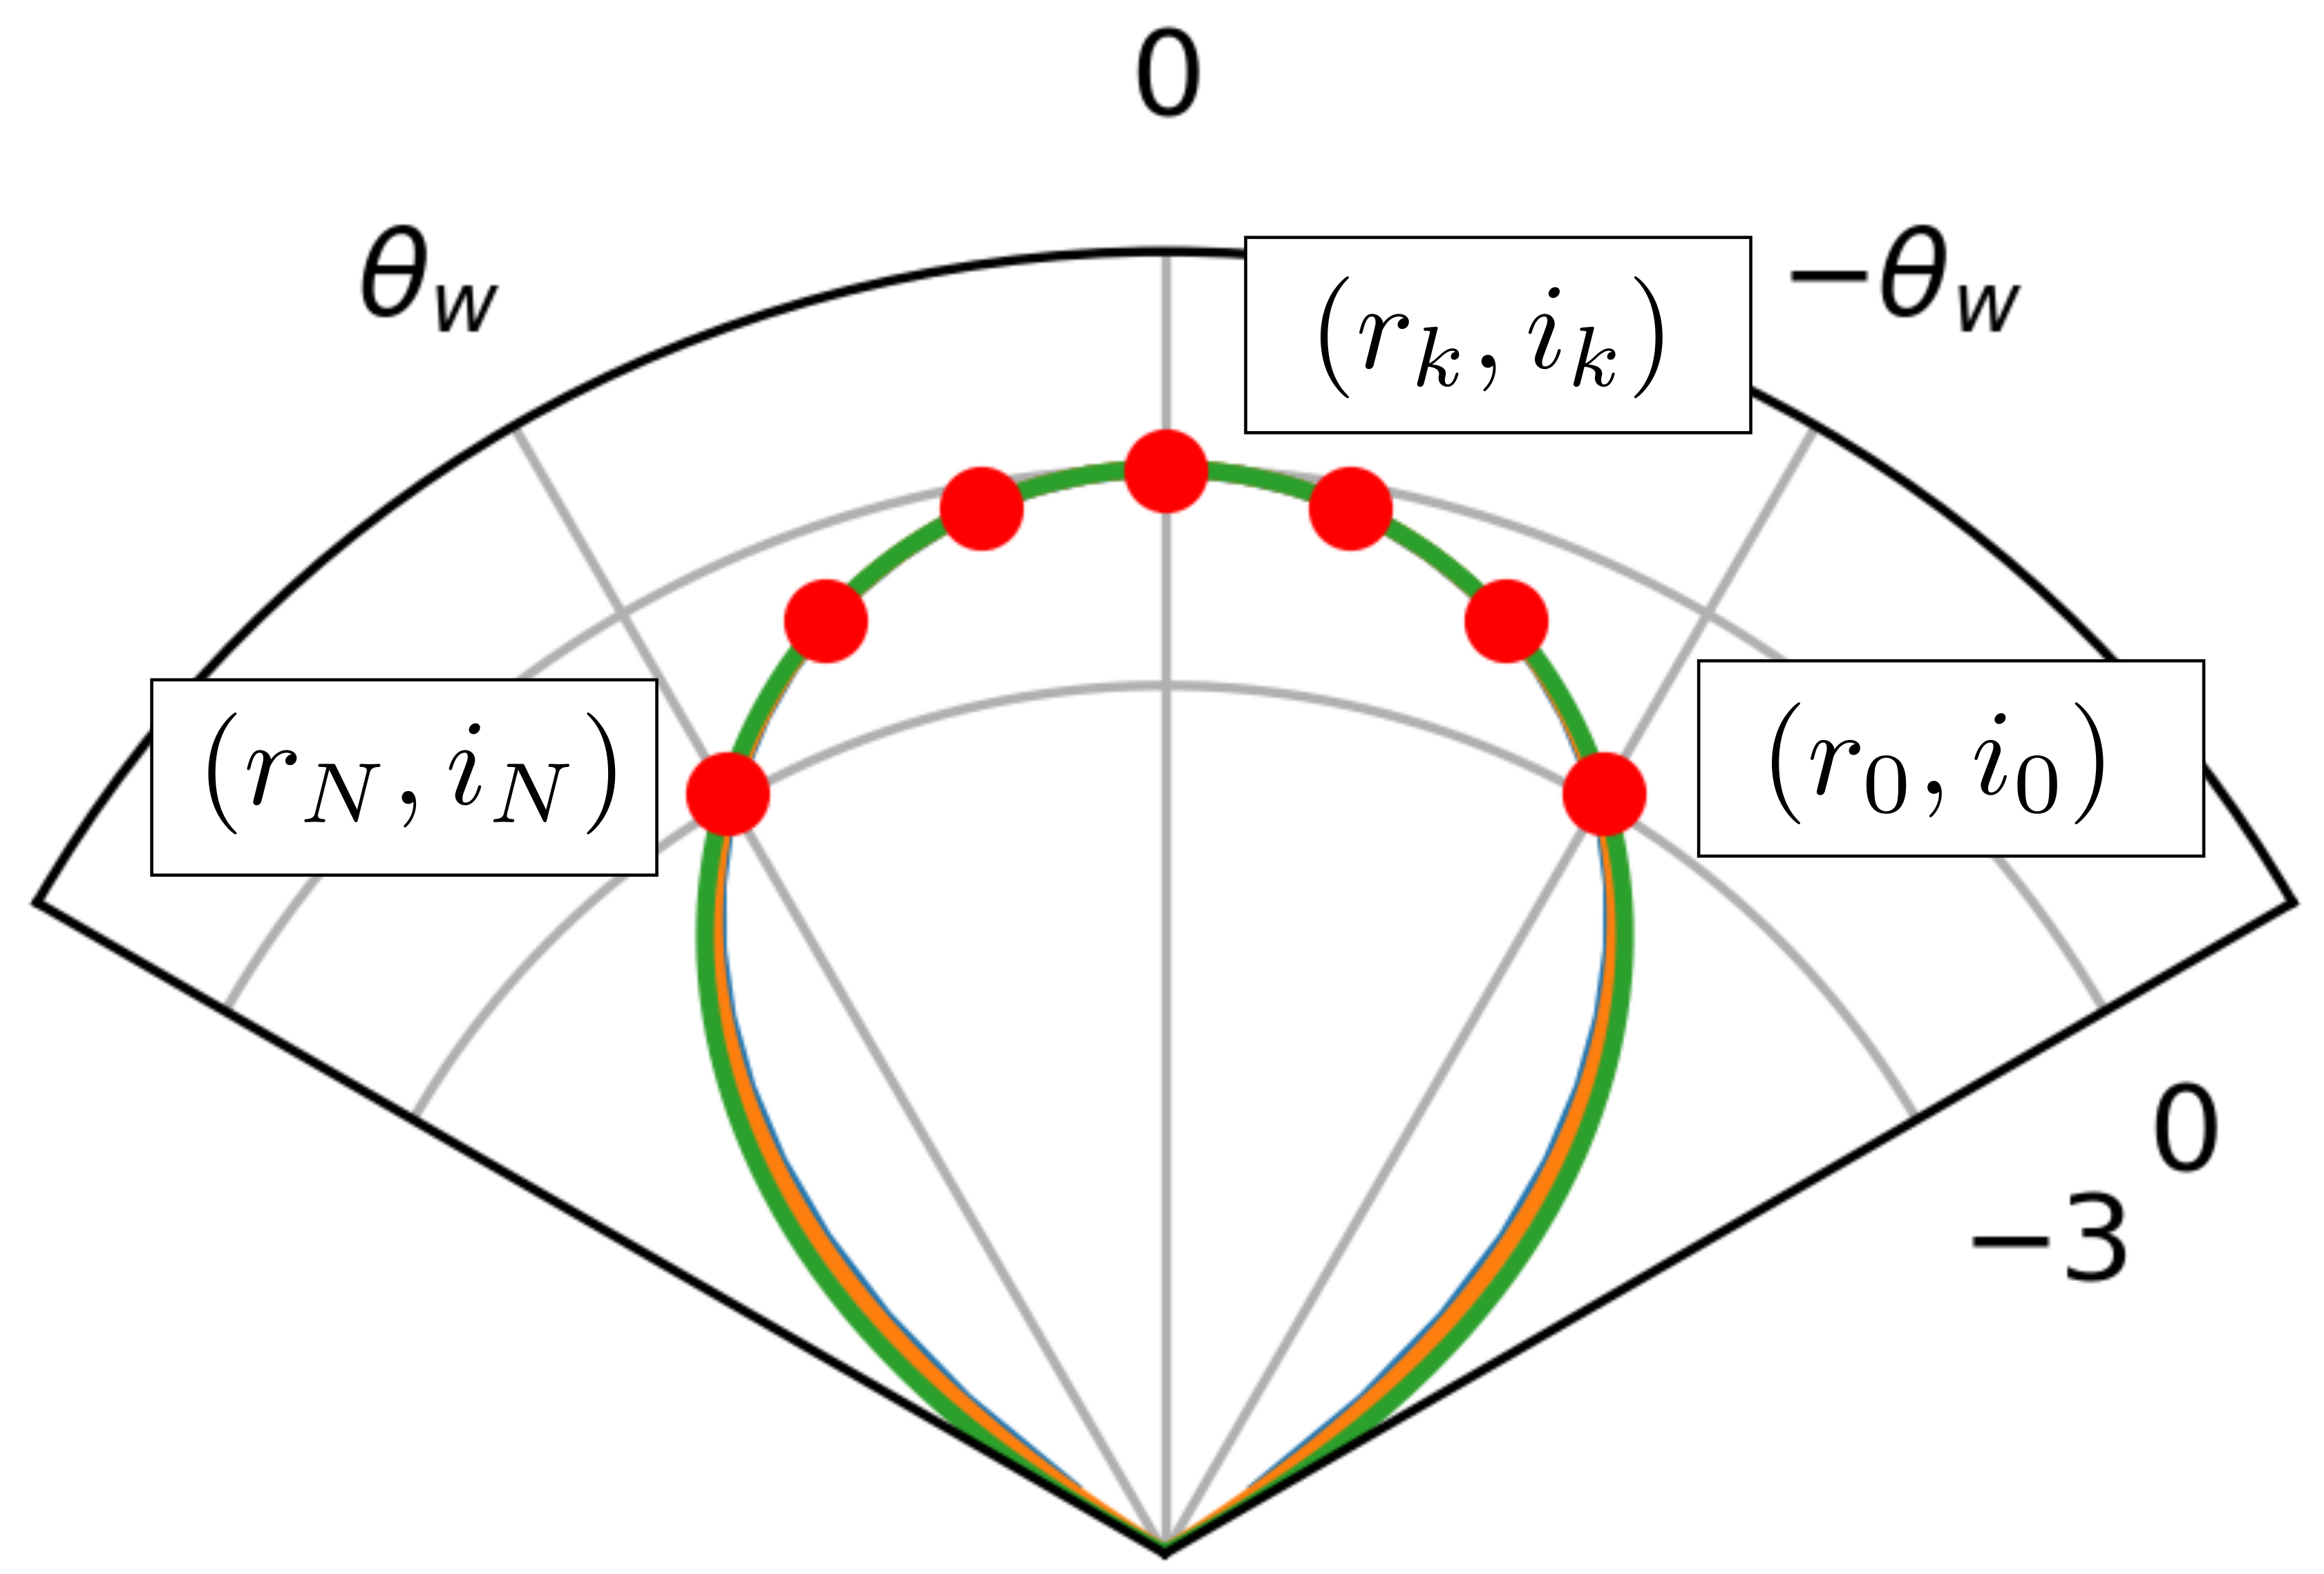
\includegraphics[width=0.75\textwidth]{src/single_beam/single_beam_sampled_annote.png}
  \caption{Beam pattern sampled}
  \label{f:bpsampled}
\end{figure}


\subsection{Gazebo Beam Output}
For each simulated beam, Gazebo should provide the set of ordered pairs of echo level and range for each ray used to sample the beam: $B= \{(r_0,EL_0),(r_1,EL_1),\ldots,(r_N,EL_n)\}$, where each echo level, $EL_k$, is the simulated echo level that takes into account
\begin{itemize}
\item The sonar equation model, including the effect of incidence angle on target strength and
\item The beam pattern function as captured by the coefficient $w_k$.
\end{itemize}



\setcounter{page}{1}
\bibliographystyle{IEEEtran}
\bibliography{bbing_master}

\end{document}
